\label{fs-formalism}

\subsection{Reference streaming model}

\begin{definition}{Reference stream processing system}
is a tuple of $(\Gamma,D)$, where $\Gamma$ is a set of all possible data flow elements, and $D\subseteq{\Gamma\times\Gamma}$ is a binary relation on it. Pair $(x,y)\in{D}$ if $y$ can be generated from $x$ within physical graph. We assume that all user-defined operations are pure.
\end{definition}

Within our model, one can define a streaming system using only data flow elements and business logic. However, without the notion of time, we cannot observe any processing progress. Let $\tau\in{\mathbb{N}}$ be an exact global discrete time. We assume that only one event can happen at any single point in time $\tau$. Let $a_\tau\in{\Gamma}$ be the element, which enters at the time $\tau$, and $b_\tau\in{2^\Gamma}$ be the elements, which leave at the time $\tau$. Let $A_{\tau}=\{a_i\}^{\tau}_{i=1}$ be a set of all input elements by the time $\tau$ and ${B}_\tau=\bigcup\limits_{i=1}^{\tau}{b_i}$ be a set of all output elements. $b_\tau$ is a set because some elements must be released atomically. 

\begin{definition}{A reference working set}
$\widehat{W}_\tau\subseteq{\Gamma}$ at the time $\tau$ is the set of elements, which are currently in the reference system:

$\widehat{W}_0=\emptyset$:

$\widehat{W}_{\tau+1}=\begin{sqcases}
\widehat{W}_{\tau}\cup{a_{\tau+1}}, & \text{or}\\
\widehat{W}_{\tau}\setminus{b_{\tau+1}}, & \text{or}\\
\widehat{W}_{\tau}\setminus{X}\cup{Y}, \forall{x\in{X}\exists{y\in{Y}}}:(x,y)\in{D} & \text{}.
\end{sqcases}$

\end{definition}

We can imagine a stream processing system as a pool, where some elements are poured in and others are poured out. Inside a pool, each element can be transformed into the other element, which can be transformed as well, and so on. Only survived elements are poured out from the pool.

% верхний индекс - что это?

\begin{definition}{System state}
$S_\tau$ at the time $\tau$ is $\widehat{W}_\tau^{\infty}$ if $A_{\infty}=\{a_i\}^{\tau}_{i=1}$.
\end{definition}

The state is a set of all data flow elements that stay in the system if we block input and wait for an infinite time. Technically, states in existing stream processing systems are not data flow elements, but as it was mentioned above, they can be presented in such a way using the drifting state model. The main purpose of the state is to accumulate information about input items.

\begin{definition}{Nullification time}
of an input element $a_\tau$ is the first moment of time when all elements that depends on $a_\tau$ are in state or released from the system, $\theta_{a_\tau}=inf(\hat{\tau}>\tau|\widehat{W}_{\hat{\tau}}\setminus{S_{\hat{\tau}}}\cap{Cl(D)(a_\tau)=\emptyset})$, where $Cl(D)$ is a transitive closure of the relation $D$.
\end{definition}

Data flow elements and their descendants cannot be in $\widehat{W}\setminus{S}$ for an infinite time by the definition of the state. Hence, for each input element $a_\tau$, there is a nullification time $\theta_{a_\tau}$, thereafter all elements, which depend on $a_\tau$, are in the system state. Since the nullification time, the input element can affect output elements only through the state.

Since we cannot observe internal transitions directly, it is convenient to limit the global time domain only to moments of output events.

\begin{definition}{Time quantization}
$\tau(t)$ is monotonic mapping from time domain restricted to only output events to global discrete time $\tau$, $\forall{t}\exists{b_{\tau(t)}}$.
\end{definition}

\begin{definition}{Probability of output element in a reference system}
$P(b_{t+1}|A_{t+1}, B_t)$ is a probability to observe output set $b$ at the time $t+1$ considering all previous input and output elements. For all output elements from the reference working set, such probability is positive,\\
$\forall{b_{t+1}:\exists{\widehat{W}_{t+1}=\widehat{W}_{t}\setminus{b_{t+1}}}} \Rightarrow P(b_{t+1}|A_{t+1}, B_t) > 0$.
\end{definition}

In classical distributed system model proposed by Chandy and Lamport~\cite{Chandy:1985:DSD:214451.214456}, a distributed system is defined as a graph of processes, which can be connected to each other via channels. Each process can generate {\em events} and send them to other processes through the channels. Global system state in this model contains processes states and channel states, e.g., elements, which are in-flight at the moment. Distributed asynchronous processing is simulated using permutations of events. 

In terms of the Chandy-Lamport model, the global state of our streaming model contains only channel states, while events are input elements, output elements, and user-defined transformations. We model the asynchronous nature of distributed processing via global discrete time, that does not determine a priori order of transformations. There is a probability to observe some specified output element, even in the reference system. However, in contrast to the Chandy-Lamport model, it is assumed that end-user is external to the system, i.e., a user is able to observe input and output elements, but not the system states. Hence, as we show further, the notion of {\em consistency} in this case should also be defined in terms of input and output.  

\subsection{Streaming model with failures}

Unfortunately, the reference stream processing system is just an abstract concept, because it does not capture possible failures of network and computational units. Failure can be expressed as a loss of the working set or its part. There is a need to extend the reference model by a recovery mechanism that allows a system to transparently pass through the failures.

% {\bf Snapshot = set!}
% P and P_{\tau}??

\begin{definition}{Stream processing system}
is a tuple of\\
$(\Gamma,D,P,F)$. $(\Gamma, D)$ defines the reference system. Snapshot $P$ is an information about system execution that is available even in case of a system failure. At time $\tau$ snapshot contains information $P_\tau$. Recovery function $F(A^{p}_\tau,P_\tau)$ provides logic for recovering of working set in case of system failures based on some set of input elements and a snapshot.
\end{definition}

\begin{definition}{Working set}
$W_\tau\subseteq{\Gamma}$ at the time $\tau$ is the set of elements, which are currently in the system:

$W_0=\emptyset$:

$W_{\tau+1}=\begin{sqcases}
W_{\tau}\cup{a_{\tau+1}}, & \text{or}\\
W_{\tau}\setminus{b_{\tau+1}}, & \text{or}\\
W_{\tau}\setminus{X}\cup{Y}, \forall{x\in{X}\exists{y\in{Y}}}:(x,y)\in{D} & \text{or}\\
F(A^{p}_\tau,P_\tau), A^{p}_\tau\subseteq{A_\tau} & \text{}.
\end{sqcases}$

\end{definition}

Working set captures the same transitions as the reference working set, but it also has a {\em recovery transition}. 

% The notions of system state and nullification time are obviously generalized to this model by substitution of $\widehat{W}_\tau$ for $W_\tau$.

\begin{definition}{Probability of output element}
$P(b_{t+1}|A_{t+1}, B_t, P_t,F)$ is a probability to observe output element $b$ at the time $t+1$ considering all previous input and output elements, current snapshot, and recovery function.
\end{definition}

% сказать явно, что такое V

\subsection{Consistency guarantees}

The reference system concept allows us to express the notion of valid execution in terms of correspondence between input and output elements. In most real cases, input and output elements are the only data that can be observed by end-user. In real distributed stream processing systems, failures and recoveries can corrupt the output, despite the fact, that in terms of a naive definition of delivery guarantees, all elements are processed exactly once. Let us demonstrate it by an example. Assume that execution graph consists of a single operation $V^{i+1}=a_\tau(1+V^{i}),V^{0}=0,V\in{S}$ and $\forall{t},b_t=V$. In case of failure and recovery, the consistency of subsequent results depends not only on further input elements but on the restored $V$ as well. If a system recovers $V$ incorrectly after a failure, the results may become inconsistent, e.g. the property of output monotonicity can be violated. For instance, if $V=0$ after recovery, but before failure it was equal to some value $q\neq{0}$, end-user will receive unexpected output, even if each input element $a_\tau$ is processed exactly once. This example is demonstrated in Figure~\ref{state-inconsistency}. 

\begin{figure}[htbp]
  \centering
  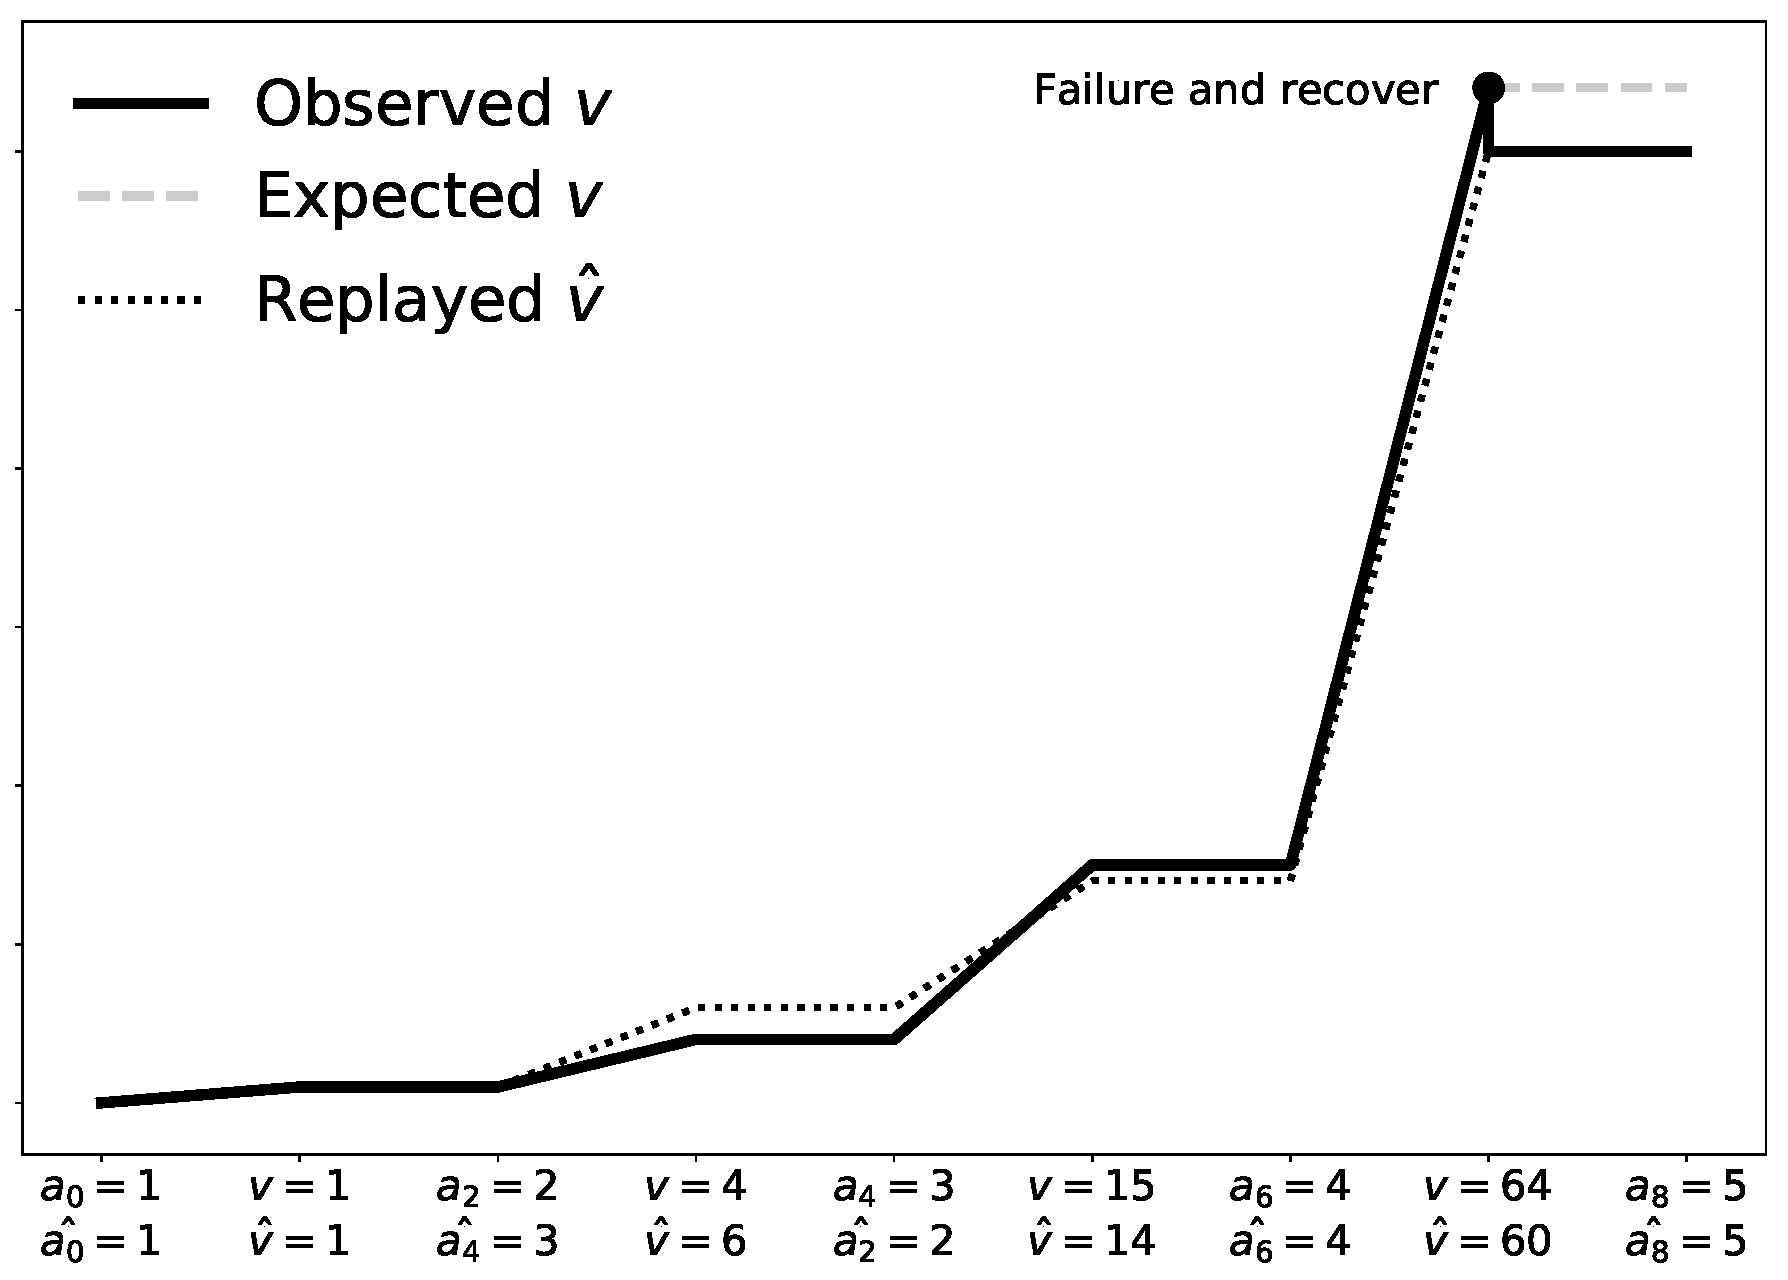
\includegraphics[width=0.48\textwidth]{pics/failure}
  \caption{Inconsistency of results after incorrect recovery}
  \label {state-inconsistency}
\end{figure}

\begin{definition}{System provides for exactly once}
if it is possible to obtain each output element $b_{t+1}$ in the reference stream processing system, i.e.,\\ 
$\forall{t} \forall{b_{t+1}}: P(b_{t+1}|A_{t+1},B_t,P_t,F)>0 \Rightarrow P(b_{t+1}|A_{t+1},B_t)>0$.
\end{definition}

\begin{definition}{System provides for at most once}
if \\
$\exists{A^{0}_{t+1}\subseteq{A_{t+1}}}$ such that \\
$\forall{t} \forall{b_{t+1}}: P(b_{t+1}|A_{t+1},B_t,P_t,F)>0 \Rightarrow P(b_{t+1}|A^{0}_{t+1},B_t)>0$.
\end{definition}

\begin{definition}{System provides for at least once}
if \\
$\exists{A^{*}_{t+1}\subseteq{2^{A_{t+1}}}}$ such that \\
$\forall{t} \forall{b_{t+1}}: P(b_{t+1}|A_{t+1},B_t,P_t,F)>0 \Rightarrow P(b_{t+1}|A^{*}_{t+1},B_t)>0$.
\end{definition}

Exactly once states that observed results cannot be distinguished from one of the possible results produced by the reference system. At most once and at least once guarantees are the relaxations of exactly once. The results within these guarantees can be obtained in the reference system, but with the assumption, that input is not completely correct. At least once can be reproduced if the input contains duplicates. At most once can be achieved in the reference system if some input elements are missed. It is important to note, that regarding at most once guarantee we require an input element to be processed atomically with all its derivatives or not processed at all. To the best of our knowledge, no one real stream processing engine supports at most once guarantee, so we cannot verify the relevancy of this assumption. It is easy to provide at most once by producing no output at all but if output is presented, at most once enforcement becomes much more difficult.  

In our formal model, the relaxations of exactly once are defined without diving into recovery mechanisms. Instead, they are described through possible input channel flaws in a reference system. This trick allows us to represent invisible system details in terms clear for a user.

We can proceed from the probability of output element to the probability of the working set through the formula of total probability:

$P(b_{t+1}|A_{t+1},B_t)=\\
\sum\limits_{W_{t+1}}P(W_{t+1}|A_{t+1},B_t)P(b_{t+1}|A_{t+1},B_t,W_{t+1})=\\
\sum\limits_{W_{t+1}}P(W_{t+1}|A_{t+1},B_t)P(b_{t+1}|W_{t+1})
$.

Hence, in order to preserve exactly once, system must preserve working set that is possible to observe in reference system, because $\forall{t} \forall{b_{t+1}} P(b_{t+1}|A_{t+1},B_t)>0$ only if $\forall{t} \exists{W_{t+1}}:P(W_{t+1}|A_{t+1},B_t)>0$.

\begin{definition}{Snapshotting mechanism $P,F$ is consistent}
if $\forall{t} \exists{A^{p}_t\subseteq{A_t}} : P(F(A^{p}_t,P_t)|A_{t+1},B_t)>0$.
\end{definition}

% MillWheel ensures that $F(\emptyset,P_t)=\widehat{W_t}$ using strong productions and deduplication.

\begin{definition}{State snapshot}
$P^{s}$ is a snapshot such that $\forall{t} P^{s}_t = S_{t_s},t_s \leq t$.
\end{definition}

A streaming system must provide for consistent state snapshotting mechanism in order to support exactly once processing by the definition. Further, we demonstrate the ways how it is done in state-of-the-art solutions, but before it, we formally show the basic motivation behind some of them. 

One of the main factors that affects a method of taking a snapshot is the amount of information that is included in the snapshot. An obvious idea is to maintain the whole $W$, like it is done in MillWheel. Some other industrial systems, like Flink and Storm, save only system state, that takes up less disk space in general. However, state snapshotting imposes additional restrictions on the snapshot structure and mechanism.

\begin{theorem}
\label{necessary_conditions}
The necessary conditions of consistent state snapshotting are:\\
1. State snapshot is taken at each time $t$ of output delivery, $\forall{D{\subseteq{\Gamma\times\Gamma}},  t\in{\mathbb{N}},b_t\in{2^{\Gamma}}}:P^{s}_t \supseteq S_t$\\
2. Input elements are stored until their nullification time, $\forall{t\in{\mathbb{N}}, a}\in{A_t \setminus A^{p}_t} : \theta_a \leq t$
\end{theorem}
\begin{sketch}
$ $\newline
1. Assume that $\exists{t\in{\mathbb{N}}},b_t\in 2^{\Gamma}$ and $S_{t}\setminus{P^{s}_t}=\{y\}$. Let $D$ be the following: $b_{t+k},b_t\in{Cl(y)}$ and $y\in{Cl(a_{t-1})}$. These scheme of $D$ captures a lot of real processing scenarios including example shown in Figure~\ref{state-inconsistency}, where $y$ can be considered as a state sum. Let system fails at $\tau_f = \tau(t)+1$. There are two options on recovery: to replay element $a_{t-1}$ or to not replay. Reprocessing of $a_{t-1}$ causes repeated output of $b_{t}$ at time $t+1$ that is impossible in a reference system, $P(b_{t+1}=b_{t}|A_{t+1},B_{t})=0$. On the other hand, without replay, expected element $b_{t+k}\in{Cl(y)}$ will never be released, because $y$ will not be restored.\\
2. Assume that $\exists{}t\in{\mathbb{N}},a \in{A_t \setminus A^{p}_t}:\theta_{a}>t$. In this case, $Cl(D)(a) \cap (W_t \setminus{S_t}) \neq \emptyset$. If system fails at time $\tau_f=\tau(t)+1$, elements $Cl(D)(a) \cap (W_t \setminus{S_t})$ cannot be restored using $A^{p}_t$ and $P^{s}_t=S_t$, because restoring requires reprocessing of element $a$.
\end{sketch}

This theorem has a direct practical implication. If a system that uses state snapshots aims at providing for exactly once, it must output elements $b_t$ only if there exists a snapshot for time $t$. It means that the lower bound of latency in the worst case in such systems is the snapshotting period together with the duration of taking a snapshot. There is a trade-off between latency and the frequency of taking snapshots because too frequent snapshotting can cause high extra load, while rare snapshots lead to high latency.

\begin{definition}{System is deterministic}
if\\ 
$\forall{t\in{\mathbb{N}}, b_{t+1}\in{2^{\Gamma}}}:P(b_{t+1}|A_{t+1},B_t)=1$.
\end{definition}

The following theorem shows that for a deterministic system the first condition of a Theorem~\ref{necessary_conditions} can be relaxed. 

\begin{theorem}
\label{determinism}
A stream processing system is able to provide exactly once if the following conditions are satisfied:\\
1. System is deterministic\\
2. State snapshot is extended with the last output element, $\forall{t\in{\mathbb{N}},b_t\in{2^{\Gamma}}}:P_t=P^{s}_t \cup b_t$\\
3. Input elements are stored until their nullification time, $\forall{t\in{\mathbb{N}}, a}\in{A_t \setminus A^{p}_t} : \theta_a \leq t$
\end{theorem}
\begin{sketch}
As in Theorem~\ref{necessary_conditions}, assume that $\exists{t\in{\mathbb{N}}},b_t\in 2^{\Gamma}$, $S_{t}\setminus{P^{s}_t}=\{y\}$, and $b_{t+k},b_t\in{Cl(y)}$ and $y\in{Cl(a_{t-1})}$. Let system fails at $\tau_f = \tau(t)+1$. The problem here is that replay of $a_{t-1}$ causes inconsistent output as it is shown in Theorem~\ref{necessary_conditions}. The property of determinism guarantees that in case of reprocessing, output elements will be the same and released in the same order. Having the last released element before the failure, we can filter out output elements, which are generated during reprocessing, but have been already released before the failure.
\end{sketch}

If a system is deterministic, it is possible to inexpensively achieve a consistent snapshotting mechanism without synchronization between taking snapshots and output elements delivery. Deterministic system can release an element $b_t$ before state snapshot $P^{s}_t=S_t$ is taken. As we show further in experiments, this relaxation is able to dramatically decrease processing latency, because there is no need to wait until the snapshot is taken in order to release output elements.

To the best of our knowledge, only micro-batching systems support the property of determinism in streaming. However, micro-batching solutions provide higher latency than pure streaming engines due to overhead on input buffering~\cite{karimov2018benchmarking}. We proposed a pure streaming model called {\em drifting state}~\cite{we2018adbis} that allows achieving both determinism and low latency. Therefore, a question arises: is it more efficient in practice to handle non-determinism by atomic snapshotting and releasing than to maintain a fair determinism in order to get exactly once? 

It is important to note that the proposed model is suitable not only for the formal analysis of the properties of exactly once but for a deeper understanding of the other aspects of stream processing. While these topics are promising as well, they are out of scope of this paper. 

\subsection{Examples}

In state-of-the-art stream processing systems $\Gamma$ contains all possible objects that can be processed inside a system. For example, in Storm, $\Gamma$ contains all possible {\em Tuples}, while in Flink all {\em StreamRecords}. Dependency relation $D$ is defined in a form of a logical graph that is commonly assumed as directed and acyclic.

\subsubsection{MillWheel}

MillWheel maintains the whole $W$ in a snapshot. Each operation saves all its input elements for deduplication and output elements for resending. There is no need to replay input elements because the system can completely restore computations using only a snapshot. {\em Strong productions} mechanism allows MillWheel to preserve exactly-once guarantee for the price of persistent updates of $P_\tau=W_\tau$ on each $\tau$~\cite{Akidau:2013:MFS:2536222.2536229}.    

\subsubsection{Flink}

Flink uses the state snapshotting mechanism. It artificially reproduces a moment $t_s$, when $\forall{a}\in{Cl^{-1}(D)(S_{t_s})}:\theta_a \leq t_s$, and saves obtained $S_{t_s}$. Flink achieves consistent state by injecting special elements called {\em checkpoints} into the input stream. Checkpoints go through the same network channels as ordinary elements and push all inverted dependencies of inputs through the system. Each operation in data flow prepares its snapshot independently at the moment of checkpoint arrival. Global snapshot is taken when checkpoint passes through the whole data flow. Flink atomicity between state snapshotting and elements delivery is preserved using the modification of 2PC protocol.

Besides overhead on snapshotting and delivery synchronization, checkpoints cause extra latency overhead because an operation with multiple inputs must wait until checkpoints arrive from each input. Only after that, an operation can safely send checkpoint further. This behavior is known as {\em checkpoints alignment}.

\subsubsection{Spark streaming}

To the best of our knowledge, spark streaming is the only state-of-the-art stream processing system that provides for deterministic results. However, an architecture based on input buffering makes it hard to achieve latency lower than several seconds~\cite{7530084, 7474816}. 
